\documentclass{standalone}
\usepackage{tikz}
\usetikzlibrary{patterns, positioning}

\begin{document}
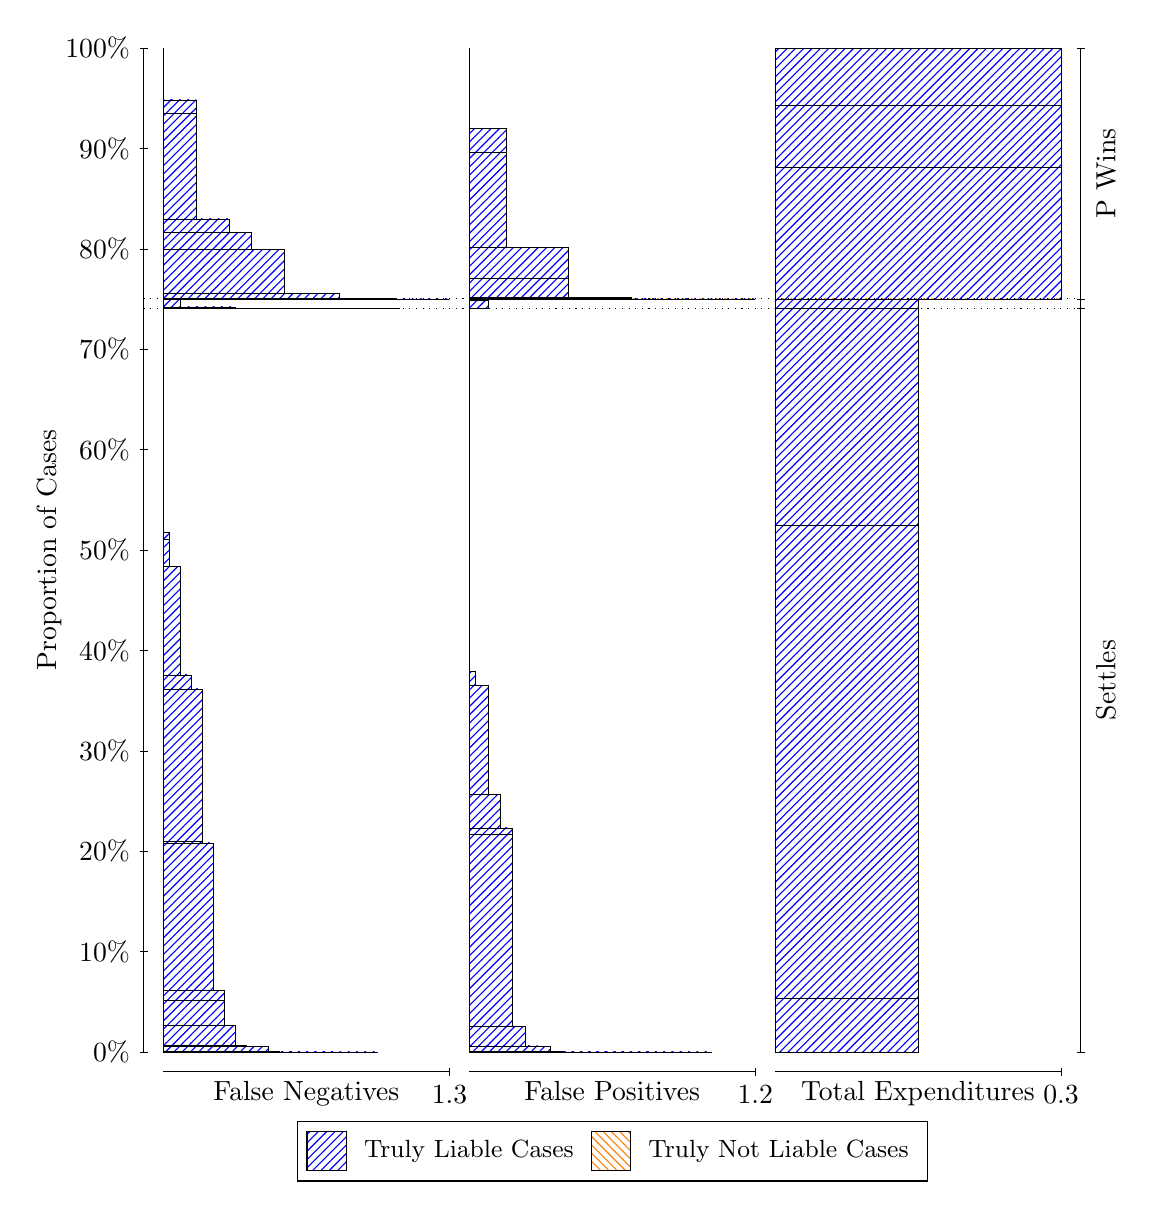
\begin{tikzpicture}
\draw[black, very thin] (1.5,1.75) -- (1.5,14.5);
\node[rotate=90, anchor=center] at (0.3, 8.125) {Proportion of Cases};
\draw[black, very thin] (1.45,1.75) -- (1.55,1.75);
\node[anchor=east] at (1.45, 1.75) {0\%};
\draw[black, very thin] (1.45,3.025) -- (1.55,3.025);
\node[anchor=east] at (1.45, 3.025) {10\%};
\draw[black, very thin] (1.45,4.3) -- (1.55,4.3);
\node[anchor=east] at (1.45, 4.3) {20\%};
\draw[black, very thin] (1.45,5.575) -- (1.55,5.575);
\node[anchor=east] at (1.45, 5.575) {30\%};
\draw[black, very thin] (1.45,6.85) -- (1.55,6.85);
\node[anchor=east] at (1.45, 6.85) {40\%};
\draw[black, very thin] (1.45,8.125) -- (1.55,8.125);
\node[anchor=east] at (1.45, 8.125) {50\%};
\draw[black, very thin] (1.45,9.4) -- (1.55,9.4);
\node[anchor=east] at (1.45, 9.4) {60\%};
\draw[black, very thin] (1.45,10.675) -- (1.55,10.675);
\node[anchor=east] at (1.45, 10.675) {70\%};
\draw[black, very thin] (1.45,11.95) -- (1.55,11.95);
\node[anchor=east] at (1.45, 11.95) {80\%};
\draw[black, very thin] (1.45,13.225) -- (1.55,13.225);
\node[anchor=east] at (1.45, 13.225) {90\%};
\draw[black, very thin] (1.45,14.5) -- (1.55,14.5);
\node[anchor=east] at (1.45, 14.5) {100\%};

\draw[black, very thin] (13.4,1.75) -- (13.4,14.5);
\draw[black, very thin] (13.35,1.75) -- (13.45,1.75);
\node[anchor=west] at (13.35, 1.75) {};
\draw[black, very thin] (13.35,11.195) -- (13.45,11.195);
\node[anchor=west] at (13.35, 11.195) {};
\draw[black, very thin] (13.35,11.315) -- (13.45,11.315);
\node[anchor=west] at (13.35, 11.315) {};
\draw[black, very thin] (13.35,14.5) -- (13.45,14.5);
\node[anchor=west] at (13.35, 14.5) {};

\draw[black, very thin, pattern color=blue, pattern=north east lines] (1.75,1.75) rectangle (4.475,1.75);
\draw[black, very thin, pattern color=blue, pattern=north east lines] (1.75,1.75) rectangle (3.916,1.75);
\draw[black, very thin, pattern color=blue, pattern=north east lines] (1.75,1.75) rectangle (3.7763,1.75);
\draw[black, very thin, pattern color=blue, pattern=north east lines] (1.75,1.75) rectangle (3.6365,1.75);
\draw[black, very thin, pattern color=blue, pattern=north east lines] (1.75,1.75) rectangle (3.3571,1.7506);
\draw[black, very thin, pattern color=blue, pattern=north east lines] (1.75,1.7506) rectangle (3.2173,1.7528);
\draw[black, very thin, pattern color=blue, pattern=north east lines] (1.75,1.7528) rectangle (3.0776,1.8172);
\draw[black, very thin, pattern color=blue, pattern=north east lines] (1.75,1.8172) rectangle (2.9378,1.8178);
\draw[black, very thin, pattern color=blue, pattern=north east lines] (1.75,1.8178) rectangle (2.9378,1.8178);
\draw[black, very thin, pattern color=blue, pattern=north east lines] (1.75,1.8178) rectangle (2.7981,1.8297);
\draw[black, very thin, pattern color=blue, pattern=north east lines] (1.75,1.8297) rectangle (2.6583,2.0883);
\draw[black, very thin, pattern color=blue, pattern=north east lines] (1.75,2.0883) rectangle (2.5186,2.4095);
\draw[black, very thin, pattern color=blue, pattern=north east lines] (1.75,2.4095) rectangle (2.5186,2.5369);
\draw[black, very thin, pattern color=blue, pattern=north east lines] (1.75,2.5369) rectangle (2.3788,4.4041);
\draw[black, very thin, pattern color=blue, pattern=north east lines] (1.75,4.4041) rectangle (2.2391,4.4226);
\draw[black, very thin, pattern color=blue, pattern=north east lines] (1.75,4.4226) rectangle (2.2391,4.4226);
\draw[black, very thin, pattern color=blue, pattern=north east lines] (1.75,4.4226) rectangle (2.2391,6.3611);
\draw[black, very thin, pattern color=blue, pattern=north east lines] (1.75,6.3611) rectangle (2.0994,6.5383);
\draw[black, very thin, pattern color=blue, pattern=north east lines] (1.75,6.5383) rectangle (1.9596,7.9217);
\draw[black, very thin, pattern color=blue, pattern=north east lines] (1.75,7.9217) rectangle (1.8199,8.2584);
\draw[black, very thin, pattern color=blue, pattern=north east lines] (1.75,8.2584) rectangle (1.8199,8.3488);
\draw[black, very thin, pattern color=orange, pattern=north west lines] (1.75,8.3488) rectangle (1.75,8.3488);
\draw[black, very thin, pattern color=blue, pattern=north east lines] (1.75,8.3488) rectangle (1.75,11.195);
\draw[black, very thin, pattern color=blue, pattern=north east lines] (1.75,11.195) rectangle (4.7545,11.195);
\draw[black, very thin, pattern color=blue, pattern=north east lines] (1.75,11.195) rectangle (4.0558,11.195);
\draw[black, very thin, pattern color=blue, pattern=north east lines] (1.75,11.195) rectangle (3.3571,11.195);
\draw[black, very thin, pattern color=blue, pattern=north east lines] (1.75,11.195) rectangle (2.6583,11.213);
\draw[black, very thin, pattern color=blue, pattern=north east lines] (1.75,11.213) rectangle (1.9596,11.315);
\draw[black, very thin, pattern color=orange, pattern=north west lines] (1.75,11.315) rectangle (1.75,11.315);
\draw[black, very thin, pattern color=blue, pattern=north east lines] (1.75,11.315) rectangle (5.3833,11.315);
\draw[black, very thin, pattern color=blue, pattern=north east lines] (1.75,11.315) rectangle (4.6846,11.316);
\draw[black, very thin, pattern color=blue, pattern=north east lines] (1.75,11.316) rectangle (4.2654,11.316);
\draw[black, very thin, pattern color=blue, pattern=north east lines] (1.75,11.316) rectangle (3.9859,11.384);
\draw[black, very thin, pattern color=blue, pattern=north east lines] (1.75,11.384) rectangle (3.5667,11.384);
\draw[black, very thin, pattern color=blue, pattern=north east lines] (1.75,11.384) rectangle (3.2872,11.938);
\draw[black, very thin, pattern color=blue, pattern=north east lines] (1.75,11.938) rectangle (2.8679,12.162);
\draw[black, very thin, pattern color=blue, pattern=north east lines] (1.75,12.162) rectangle (2.5885,12.331);
\draw[black, very thin, pattern color=blue, pattern=north east lines] (1.75,12.331) rectangle (2.1692,13.67);
\draw[black, very thin, pattern color=blue, pattern=north east lines] (1.75,13.67) rectangle (2.1692,13.842);
\draw[black, very thin, pattern color=blue, pattern=north east lines] (1.75,13.842) rectangle (1.8897,13.842);
\draw[black, very thin, pattern color=orange, pattern=north west lines] (1.75,13.842) rectangle (1.75,13.842);
\draw[black, very thin, pattern color=blue, pattern=north east lines] (1.75,13.842) rectangle (1.75,14.5);
\draw[black, very thin, pattern color=orange, pattern=north west lines] (5.6333,1.75) rectangle (8.7138,1.75);
\draw[black, very thin, pattern color=blue, pattern=north east lines] (5.6333,1.75) rectangle (8.7138,1.75);
\draw[black, very thin, pattern color=orange, pattern=north west lines] (5.6333,1.75) rectangle (8.3978,1.75);
\draw[black, very thin, pattern color=blue, pattern=north east lines] (5.6333,1.75) rectangle (8.3978,1.75);
\draw[black, very thin, pattern color=orange, pattern=north west lines] (5.6333,1.75) rectangle (8.0819,1.75);
\draw[black, very thin, pattern color=blue, pattern=north east lines] (5.6333,1.75) rectangle (8.0819,1.75);
\draw[black, very thin, pattern color=blue, pattern=north east lines] (5.6333,1.75) rectangle (7.9239,1.75);
\draw[black, very thin, pattern color=orange, pattern=north west lines] (5.6333,1.75) rectangle (7.7659,1.75);
\draw[black, very thin, pattern color=blue, pattern=north east lines] (5.6333,1.75) rectangle (7.7659,1.75);
\draw[black, very thin, pattern color=blue, pattern=north east lines] (5.6333,1.75) rectangle (7.608,1.75);
\draw[black, very thin, pattern color=orange, pattern=north west lines] (5.6333,1.75) rectangle (7.45,1.75);
\draw[black, very thin, pattern color=blue, pattern=north east lines] (5.6333,1.75) rectangle (7.45,1.75);
\draw[black, very thin, pattern color=blue, pattern=north east lines] (5.6333,1.75) rectangle (7.292,1.75);
\draw[black, very thin, pattern color=orange, pattern=north west lines] (5.6333,1.75) rectangle (7.1341,1.75);
\draw[black, very thin, pattern color=blue, pattern=north east lines] (5.6333,1.75) rectangle (7.1341,1.7501);
\draw[black, very thin, pattern color=orange, pattern=north west lines] (5.6333,1.7501) rectangle (7.1341,1.7501);
\draw[black, very thin, pattern color=blue, pattern=north east lines] (5.6333,1.7501) rectangle (7.1341,1.7505);
\draw[black, very thin, pattern color=blue, pattern=north east lines] (5.6333,1.7505) rectangle (6.9761,1.7506);
\draw[black, very thin, pattern color=orange, pattern=north west lines] (5.6333,1.7506) rectangle (6.8181,1.7506);
\draw[black, very thin, pattern color=blue, pattern=north east lines] (5.6333,1.7506) rectangle (6.8181,1.7547);
\draw[black, very thin, pattern color=blue, pattern=north east lines] (5.6333,1.7547) rectangle (6.6601,1.8191);
\draw[black, very thin, pattern color=blue, pattern=north east lines] (5.6333,1.8191) rectangle (6.5022,1.8275);
\draw[black, very thin, pattern color=blue, pattern=north east lines] (5.6333,1.8275) rectangle (6.3442,1.8283);
\draw[black, very thin, pattern color=blue, pattern=north east lines] (5.6333,1.8283) rectangle (6.3442,2.0766);
\draw[black, very thin, pattern color=orange, pattern=north west lines] (5.6333,2.0766) rectangle (6.1862,2.0766);
\draw[black, very thin, pattern color=blue, pattern=north east lines] (5.6333,2.0766) rectangle (6.1862,4.5165);
\draw[black, very thin, pattern color=blue, pattern=north east lines] (5.6333,4.5165) rectangle (6.1862,4.5961);
\draw[black, very thin, pattern color=blue, pattern=north east lines] (5.6333,4.5961) rectangle (6.0283,5.0232);
\draw[black, very thin, pattern color=blue, pattern=north east lines] (5.6333,5.0232) rectangle (5.8703,6.4066);
\draw[black, very thin, pattern color=blue, pattern=north east lines] (5.6333,6.4066) rectangle (5.7123,6.5838);
\draw[black, very thin, pattern color=blue, pattern=north east lines] (5.6333,6.5838) rectangle (5.6333,11.195);
\draw[black, very thin, pattern color=orange, pattern=north west lines] (5.6333,11.195) rectangle (5.8703,11.195);
\draw[black, very thin, pattern color=blue, pattern=north east lines] (5.6333,11.195) rectangle (5.8703,11.297);
\draw[black, very thin, pattern color=blue, pattern=north east lines] (5.6333,11.297) rectangle (5.6333,11.315);
\draw[black, very thin, pattern color=orange, pattern=north west lines] (5.6333,11.315) rectangle (9.2667,11.315);
\draw[black, very thin, pattern color=blue, pattern=north east lines] (5.6333,11.315) rectangle (9.2667,11.315);
\draw[black, very thin, pattern color=orange, pattern=north west lines] (5.6333,11.315) rectangle (8.4768,11.315);
\draw[black, very thin, pattern color=blue, pattern=north east lines] (5.6333,11.315) rectangle (8.4768,11.315);
\draw[black, very thin, pattern color=blue, pattern=north east lines] (5.6333,11.315) rectangle (8.4768,11.315);
\draw[black, very thin, pattern color=orange, pattern=north west lines] (5.6333,11.315) rectangle (7.687,11.315);
\draw[black, very thin, pattern color=blue, pattern=north east lines] (5.6333,11.315) rectangle (7.687,11.323);
\draw[black, very thin, pattern color=blue, pattern=north east lines] (5.6333,11.323) rectangle (7.687,11.338);
\draw[black, very thin, pattern color=orange, pattern=north west lines] (5.6333,11.338) rectangle (7.213,11.338);
\draw[black, very thin, pattern color=blue, pattern=north east lines] (5.6333,11.338) rectangle (7.213,11.338);
\draw[black, very thin, pattern color=orange, pattern=north west lines] (5.6333,11.338) rectangle (6.8971,11.338);
\draw[black, very thin, pattern color=blue, pattern=north east lines] (5.6333,11.338) rectangle (6.8971,11.575);
\draw[black, very thin, pattern color=blue, pattern=north east lines] (5.6333,11.575) rectangle (6.8971,11.973);
\draw[black, very thin, pattern color=orange, pattern=north west lines] (5.6333,11.973) rectangle (6.4232,11.973);
\draw[black, very thin, pattern color=blue, pattern=north east lines] (5.6333,11.973) rectangle (6.4232,11.973);
\draw[black, very thin, pattern color=blue, pattern=north east lines] (5.6333,11.973) rectangle (6.1072,13.172);
\draw[black, very thin, pattern color=blue, pattern=north east lines] (5.6333,13.172) rectangle (6.1072,13.484);
\draw[black, very thin, pattern color=orange, pattern=north west lines] (5.6333,13.484) rectangle (5.6333,13.484);
\draw[black, very thin, pattern color=blue, pattern=north east lines] (5.6333,13.484) rectangle (5.6333,14.5);
\draw[black, very thin, pattern color=orange, pattern=north west lines] (9.5167,1.75) rectangle (11.333,1.75);
\draw[black, very thin, pattern color=blue, pattern=north east lines] (9.5167,1.75) rectangle (11.333,2.4349);
\draw[black, very thin, pattern color=orange, pattern=north west lines] (9.5167,2.4349) rectangle (11.333,2.4349);
\draw[black, very thin, pattern color=blue, pattern=north east lines] (9.5167,2.4349) rectangle (11.333,8.4336);
\draw[black, very thin, pattern color=orange, pattern=north west lines] (9.5167,8.4336) rectangle (11.333,8.4336);
\draw[black, very thin, pattern color=blue, pattern=north east lines] (9.5167,8.4336) rectangle (11.333,11.195);
\draw[black, very thin, pattern color=orange, pattern=north west lines] (9.5167,11.195) rectangle (11.333,11.195);
\draw[black, very thin, pattern color=blue, pattern=north east lines] (9.5167,11.195) rectangle (11.333,11.315);
\draw[black, very thin, pattern color=orange, pattern=north west lines] (9.5167,11.315) rectangle (13.15,11.315);
\draw[black, very thin, pattern color=blue, pattern=north east lines] (9.5167,11.315) rectangle (13.15,12.983);
\draw[black, very thin, pattern color=orange, pattern=north west lines] (9.5167,12.983) rectangle (13.15,12.983);
\draw[black, very thin, pattern color=blue, pattern=north east lines] (9.5167,12.983) rectangle (13.15,13.774);
\draw[black, very thin, pattern color=orange, pattern=north west lines] (9.5167,13.774) rectangle (13.15,13.774);
\draw[black, very thin, pattern color=blue, pattern=north east lines] (9.5167,13.774) rectangle (13.15,14.5);
\draw[black, dotted] (1.5,11.195) -- (13.4,11.195);
\draw[black, dotted] (1.5,11.315) -- (13.4,11.315);
\draw[black, very thin] (1.75,1.5) -- (5.3833,1.5);
\node[anchor=north] at (3.5667, 1.5) {False Negatives};
\draw[black, very thin] (5.3833,1.45) -- (5.3833,1.55);
\node[anchor=north] at (5.3833, 1.45) {1.3};

\draw[black, very thin] (5.6333,1.5) -- (9.2667,1.5);
\node[anchor=north] at (7.45, 1.5) {False Positives};
\draw[black, very thin] (9.2667,1.45) -- (9.2667,1.55);
\node[anchor=north] at (9.2667, 1.45) {1.2};

\draw[black, very thin] (9.5167,1.5) -- (13.15,1.5);
\node[anchor=north] at (11.333, 1.5) {Total Expenditures};
\draw[black, very thin] (13.15,1.45) -- (13.15,1.55);
\node[anchor=north] at (13.15, 1.45) {0.3};

\node[black, centered, rotate=90] at (13.72, 6.4725) {Settles};

\node[black, centered, rotate=90] at (13.72, 12.908) {P Wins};

\draw (7.449999999999999,1.5) node[draw=none] (baseCoordinate) {};
\begin{scope}[align=center]
        \matrix[scale=0.5, draw=black, below=0.5cm of baseCoordinate, nodes={draw}, column sep=0.1cm]{
            \node[rectangle, draw, minimum width=0.5cm, minimum height=0.5cm, pattern=north east lines, pattern color=blue] {}; &
            \node[draw=none, font=\small] (B) {Truly Liable Cases}; &
            \node[rectangle, draw, minimum width=0.5cm, minimum height=0.5cm, pattern=north west lines, pattern color=orange] {}; &
            \node[draw=none, font=\small] (B) {Truly Not Liable Cases}; \\
            };
\end{scope}

\end{tikzpicture}
\end{document}